%%%%%%%%%%%%%%%%%%%%%%%%%%%%%%%%%%%%%%%%%%%%%%%%%%%%%%%
% A template for Wiley article submissions developed by 
% Overleaf for the Overleaf-Wiley pilot which ran 
% during 2017 and 2018.
% 
% This template is no longer supported, but is provided
% for historical reference. Last updated January 2019.
%
% Please note that whilst this template provides a 
% preview of the typeset manuscript for submission, it 
% will not necessarily be the final publication layout.
%
% Document class options:
% =======================
% blind: Anonymise all author, affiliation, correspondence
%        and funding information.
%
% lineno: Adds line numbers.
%
% serif: Sets the body font to be serif. 
%
% twocolumn: Sets the body text in two-column layout. 
% 
% num-refs: Uses numerical citation and references style 
%           (Vancouver-authoryear).
%
% alpha-refs: Uses author-year citation and references style
%             (rss).
%
% Using other bibliography styles:
% =======================
%
% To specify a different bibiography style
%
% 1) Do not use either num-refs or alpha-refs in documentclass.
% 2) Load natbib package with the options set as needed.
% 3) Use the \bibliographystyle command to specify the style
% 
% Included NJD styles are: 
%   WileyNJD-ACS
%   WileyNJD-AMA
%   WileyNJD-AMS
%   WileyNJD-APA
%   WileyNJD-Harvard
%   WileyNJD-VANCOUVER
%
% or you may upload an alternative .bst file 
% (if requested by the journal).
%
% Examples:
% =======================
%% Example: Using numerical, sort-by-authors citations.
\documentclass[num-refs]{wiley-article}

%% Example: Using author-year citations and anonymising submission
% \documentclass[blind,alpha-refs]{wiley-article}

%% Example: Using unsrtnat for numerical, in-sequence citations
% \documentclass{wiley-article}
% \usepackage[numbers]{natbib}
% \bibliographystyle{unsrtnat}

%% Example: Using WileyNJD-AMA reference style and superscript
%%          citations, two-column and serif fonts for AIChE
% \documentclass[serif,twocolumn,lineno]{wiley-article}
% \usepackage[super]{natbib}
% \bibliographystyle{WileyNJD-AMA}
% \makeatletter
% \renewcommand{\@biblabel}[1]{#1.}
% \makeatother

% Add additional packages here if required
\usepackage{siunitx}

% Update article type if known
\papertype{Original Article}
% Include section in journal if known, otherwise delete
\paperfield{Journal Section}

\title{This is my title}

% List abbreviations here, if any. Please note that it is preferred that abbreviations be defined at the first instance they appear in the text, rather than creating an abbreviations list.
\abbrevs{ABC, a black cat; DEF, doesn't ever fret; GHI, goes home immediately.}

% Include full author names and degrees, when required by the journal.
% Use the \authfn to add symbols for additional footnotes and present addresses, if any. Usually start with 1 for notes about author contributions; then continuing with 2 etc if any author has a different present address.
\author[1\authfn{1}]{Author One PhD}
\author[2\authfn{1}]{Author A.~Two MD}
\author[2\authfn{2}]{Author Three PhD}
\author[2]{Author B.~Four}

\contrib[\authfn{1}]{Equally contributing authors.}

% Include full affiliation details for all authors
\affil[1]{Department, Institution, City, State or Province, Postal Code, Country}
\affil[2]{Department, Institution, City, State or Province, Postal Code, Country}

\corraddress{Author One PhD, Department, Institution, City, State or Province, Postal Code, Country}
\corremail{correspondingauthor@email.com}

\presentadd[\authfn{2}]{Department, Institution, City, State or Province, Postal Code, Country}

\fundinginfo{Funder One, Funder One Department, Grant/Award Number: 123456, 123457 and 123458; Funder Two, Funder Two Department, Grant/Award Number: 123459}

% Include the name of the author that should appear in the running header
\runningauthor{Author One et al.}

\begin{document}

\begin{frontmatter}
\maketitle

\begin{abstract}
This is a generic template designed for use by multiple journals, which includes several options for customization. Please consult the author guidelines for the journal to which you are submitting in order to confirm that your manuscript will comply with the journal's requirements. Please replace this text with your abstract.

% Please include a maximum of seven keywords
\keywords{keyword 1, \emph{keyword 2}, keyword 3, keyword 4, keyword 5, keyword 6, keyword 7}
\end{abstract}
\end{frontmatter}

\section{First Level Heading}
Please lay out your article using the section headings and example objects below, and remember to delete all help text prior to submitting your article to the journal.

\begin{figure}[bt]
\centering
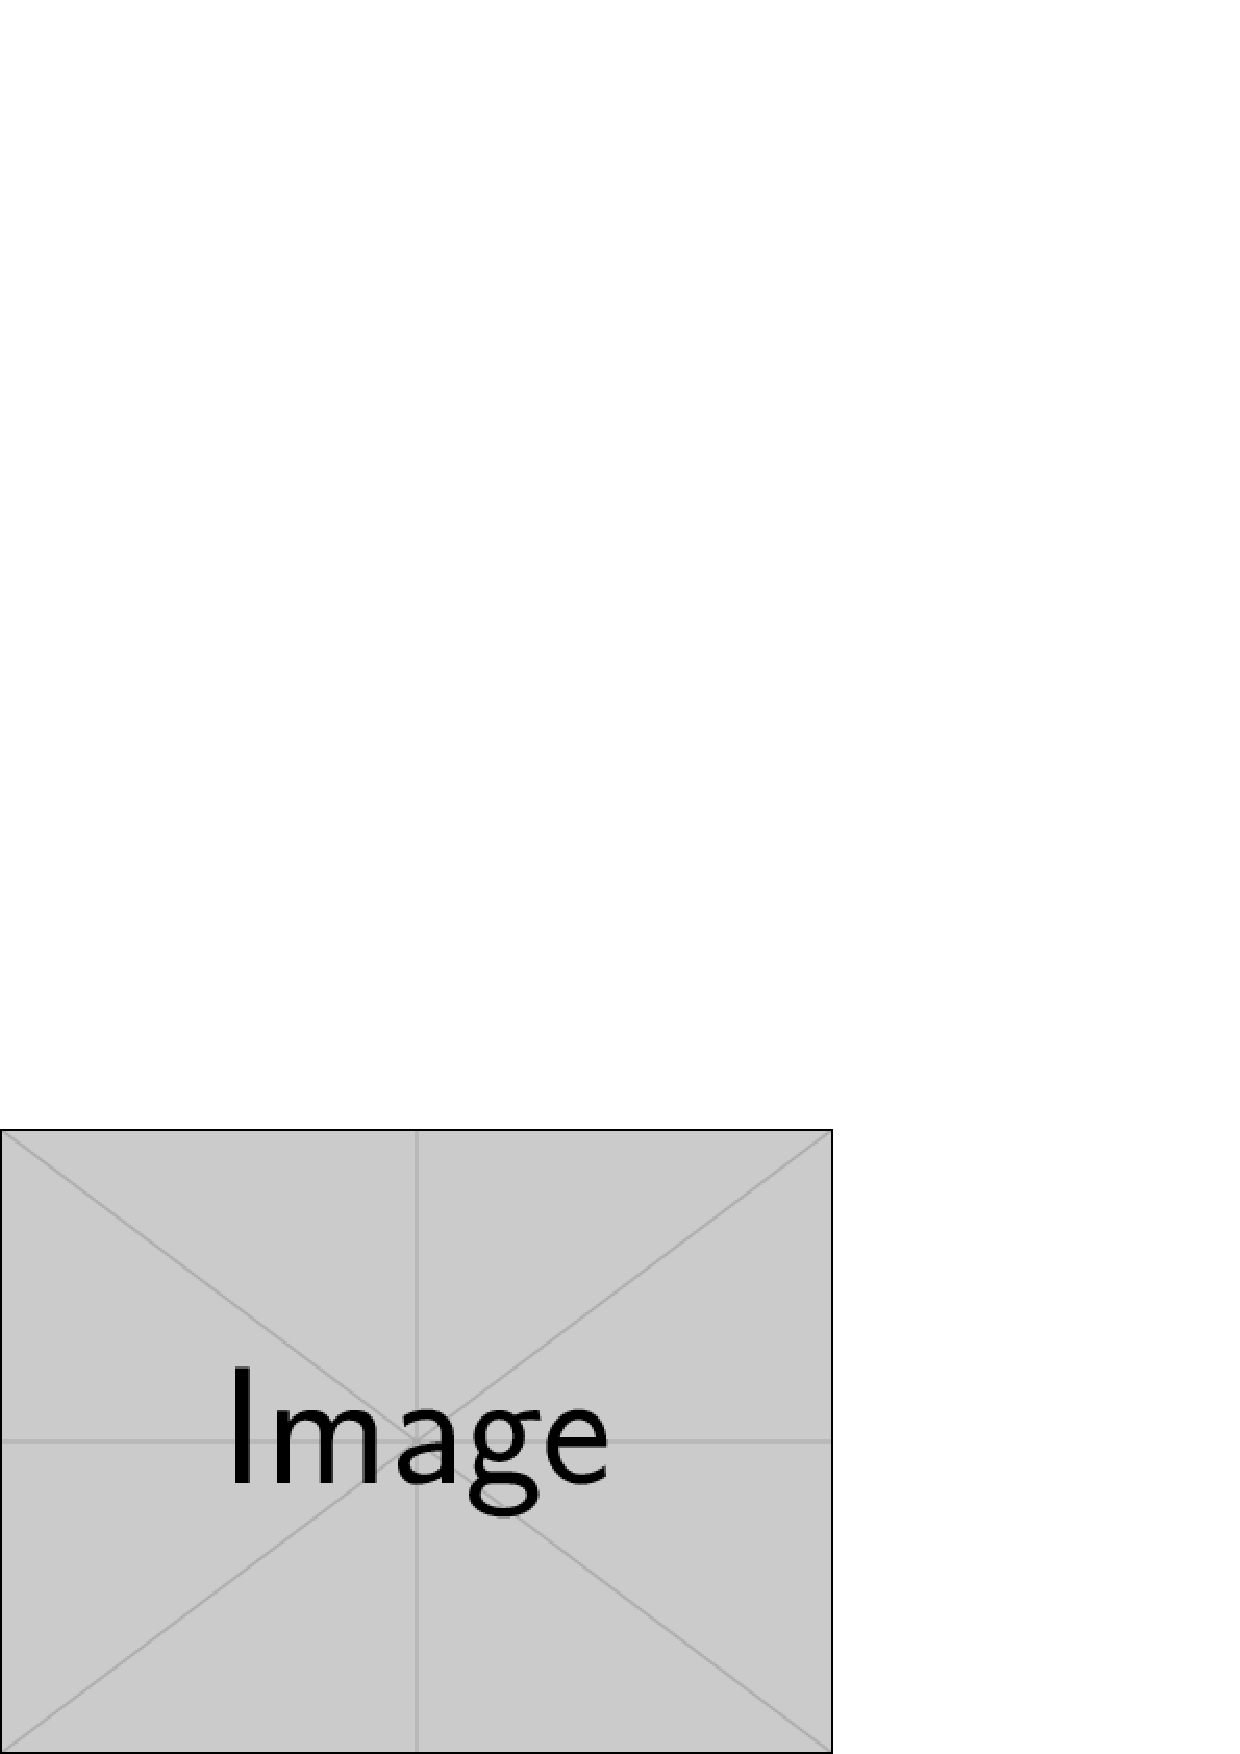
\includegraphics[width=6cm]{example-image-rectangle}
\caption{Although we encourage authors to send us the highest-quality figures possible, for peer-review purposes we can accept a wide variety of formats, sizes, and resolutions. Legends should be concise but comprehensive -- the figure and its legend must be understandable without reference to the text. Include definitions of any symbols used and define/explain all abbreviations and units of measurement.}
\end{figure}

\subsection{Second Level Heading}
If data, scripts or other artefacts used to generate the analyses presented in the article are available via a publicly available data repository, please include a reference to the location of the material within the article.

% Equations should be inserted using standard LaTeX equation and eqnarray environments, not as graphics, and should be set in the main text
This is an equation, numbered
\begin{equation}
\int_0^{+\infty}e^{-x^2}dx=\frac{\sqrt{\pi}}{2}
\end{equation}
And one that is not numbered
\begin{equation*}
e^{i\pi}=-1
\end{equation*}

\subsection{Document class options}

The \texttt{wiley-article} document class offers the following options:

\begin{description}
\item[\texttt{blind}] Anonymise all author, affiliation, correspondence
       and funding information.

\item[\texttt{lineno}] Adds line numbers.

\item[\texttt{serif}] Sets the body font to be serif.

\item[\texttt{twocolumn}] Sets the body text in two-column layout.

\item[\texttt{num-refs}] Uses the numerical Vancouver bibliography style; see section \ref{sec:bibstyles}.

\item[\texttt{alpha-refs}] Uses the author-year RSS bibliography style; see section \ref{sec:bibstyles}.
\end{description}

\subsection{Adding Citations and a References List}
\label{sec:bibstyles}

Please use a \verb|.bib| file to store your references. When using Overleaf to prepare your manuscript, you can upload a \verb|.bib| file or import your Mendeley or Zotero library directly as a \verb|.bib| file via the Add Files menu. You can then cite entries from it, like this: \cite{urmson2008autonomous,lees2010theoretical} and \cite{geiger2012we}. Just remember to specify a bibliography style, as well as the filename of the \verb|.bib|.

You can find a video tutorial here to learn more about BibTeX: \url{https://www.overleaf.com/help/97-how-to-include-a-bibliography-using-bibtex}.

This template provides two \verb|\documentclass| options for the citation and reference list style: 
\begin{description}
\item[Numerical style] Use \verb|\documentclass[...,num-refs]{wiley-article}| (Vancouver style)
\item[Author-year style] Use \verb|\documentclass[...,alpha-refs]{wiley-article}| (RSS style)
\end{description}

If you are submitting to a journal that uses neither of the above, then instead of specifying one of these options in the document class you should use  \verb|\bibliographystyle| to specify the appropriate \verb|WileyNJD-...| style, and load the \verb|natbib| with the appropriate options as needed. If the journal provides you with an alternative .bst file to use, please upload this first, and then specify it with the \verb|\bibliographystyle| as above.

\subsection{Usage Examples of \texttt{wiley-article} Options}

\begin{enumerate}
\item Using numerical, sort-by-authors citations:
\begin{verbatim}
\documentclass[num-refs]{wiley-article}
\end{verbatim}

\item Anonymised submission using author-year citations:
\begin{verbatim}
\documentclass[blind,alpha-refs]{wiley-article}
\end{verbatim}

\item Using \texttt{unsrtnat} for numerical, in-sequence citations:
\begin{verbatim}
\documentclass{wiley-article}
\usepackage[numbers]{natbib}
\bibliographystyle{unsrtnat}
\end{verbatim}

\item Using the \texttt{WileyNJD-AMA} reference style and superscript citations, two-column and serif fonts, for submission to AIChE:

\begin{verbatim}
\documentclass[serif,twocolumn]{wiley-article}
\usepackage[super]{natbib}
\bibliographystyle{WileyNJD-AMA}
\makeatletter
\renewcommand{\@biblabel}[1]{#1.}
\makeatother
\end{verbatim}

\end{enumerate}

\subsubsection{Third Level Heading}
Supporting information will be included with the published article. For submission any supporting information should be supplied as separate files but referred to in the text.

Appendices will be published after the references. For submission they should be supplied as separate files but referred to in the text.

\paragraph{Fourth Level Heading}
% Here are examples of quotes and epigraphs.
\begin{quote}
The significant problems we have cannot be solved at the same level of thinking with which we created them.\endnote{Albert Einstein said this.}
\end{quote}

\begin{epigraph}{Albert Einstein}
Anyone who has never made a mistake has never tried anything new.
\end{epigraph}

\subparagraph{Fifth level heading}
Measurements should be given in SI or SI-derived units.
Chemical substances should be referred to by the generic name only. Trade names should not be used. Drugs should be referred to by their generic names. If proprietary drugs have been used in the study, refer to these by their generic name, mentioning the proprietary name, and the name and location of the manufacturer, in parentheses.

\begin{table}[bt]
\caption{This is a table. Tables should be self-contained and complement, but not duplicate, information contained in the text. They should be not be provided as images. Legends should be concise but comprehensive � the table, legend and footnotes must be understandable without reference to the text. All abbreviations must be defined in footnotes.}
\begin{threeparttable}
\begin{tabular}{lccrr}
\headrow
\thead{Variables} & \thead{JKL ($\boldsymbol{n=30}$)} & \thead{Control ($\boldsymbol{n=40}$)} & \thead{MN} & \thead{$\boldsymbol t$ (68)}\\
Age at testing & 38 & 58 & 504.48 & 58 ms\\
Age at testing & 38 & 58 & 504.48 & 58 ms\\
Age at testing & 38 & 58 & 504.48 & 58 ms\\
Age at testing & 38 & 58 & 504.48 & 58 ms\\
\hiderowcolors
stop alternating row colors from here onwards\\
Age at testing & 38 & 58 & 504.48 & 58 ms\\
Age at testing & 38 & 58 & 504.48 & 58 ms\\
\hline  % Please only put a hline at the end of the table
\end{tabular}

\begin{tablenotes}
\item JKL, just keep laughing; MN, merry noise.
\end{tablenotes}
\end{threeparttable}
\end{table}

\section*{acknowledgements}
Acknowledgements should include contributions from anyone who does not meet the criteria for authorship (for example, to recognize contributions from people who provided technical help, collation of data, writing assistance, acquisition of funding, or a department chairperson who provided general support), as well as any funding or other support information.

\section*{conflict of interest}
You may be asked to provide a conflict of interest statement during the submission process. Please check the journal's author guidelines for details on what to include in this section. Please ensure you liaise with all co-authors to confirm agreement with the final statement.

\section*{Supporting Information}

Supporting information is information that is not essential to the article, but provides greater depth and background. It is hosted online and appears without editing or typesetting. It may include tables, figures, videos, datasets, etc. More information can be found in the journal's author guidelines or at \url{http://www.wileyauthors.com/suppinfoFAQs}. Note: if data, scripts, or other artefacts used to generate the analyses presented in the paper are available via a publicly available data repository, authors should include a reference to the location of the material within their paper.

\printendnotes

% Submissions are not required to reflect the precise reference formatting of the journal (use of italics, bold etc.), however it is important that all key elements of each reference are included.
\bibliography{sample}

\begin{biography}[example-image-1x1]{A.~One}
Please check with the journal's author guidelines whether author biographies are required. They are usually only included for review-type articles, and typically require photos and brief biographies (up to 75 words) for each author.
\bigskip
\bigskip
\end{biography}

\graphicalabstract{example-image-1x1}{Please check the journal's author guildines for whether a graphical abstract, key points, new findings, or other items are required for display in the Table of Contents.}

\end{document}